\section{事前実験2}
\label{sec:PreExperimentTwo}
事前実験2では,送られてきた32個の値を一定回数足し合わせて送り返すプログラムにおいて,TCP/IPによる通信を用いる場合と提案手法を用いる場合の単位時間あたりの演算性能を比較した.

\subsection{事前実験2用のプログラム}
事前実験2用のプログラムとして,クライアントから送られてきた32個の値を一定回数足し合わせて送り返すプログラムを作成した(図\ref{fig:PreExperimentTwo}).DPDKのRun-to-Completionモデルで実行する処理は受信したパケットに含まれる32個の値を足し合わせる処理である.このプログラムはTCP/IPによる通信を用いるものと提案手法を用いるものの2種類を作成した.

\begin{figure}[htb]
  \centering
  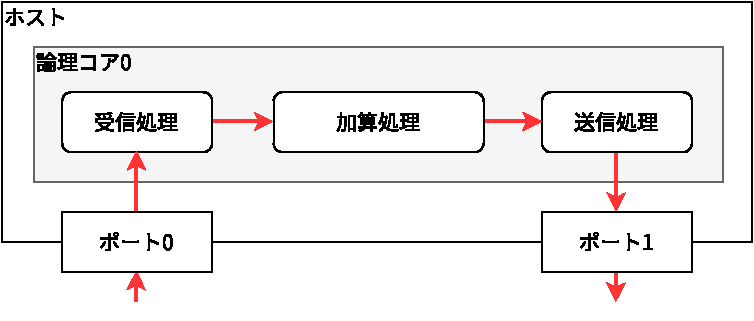
\includegraphics[width=\columnwidth]{pictures/PreExperimentTwo.pdf}
  \caption{事前実験2用のプログラム}
  \label{fig:PreExperimentTwo}
\end{figure}

\subsection{実験環境}
事前実験2で用いたネットワーク構成は事前実験1で用いたもの(図\ref{fig:PreExperimentNetwork})と同じである.ただし,クライアントにはパケットサイズが64バイトのパケットを送信レート100\%で送信し続ける自作プログラムを用いた.送信されるパケットのペイロードは要素数が32でデータ型がuint16\_tの配列である.なお,事前評価2で用いた計算機の性能は事前実験1で用いたもの(表\ref{tab:MachineSpec})と同じである.

\subsection{実験結果・考察}
事前実験2の結果を図\ref{fig:PreEvaluationTwoResult}に示す.このグラフの横軸は受信した32個の値を足し合わせる回数,縦軸は単位時間あたりの演算性能を表している.また,青はTCP/IPによる通信を用いた場合,赤は提案手法を用いた場合の結果である.グラフより,提案手法を用いた場合の演算性能はTCP/IPによる通信を用いた場合に比べて,足し合わせる回数が1回の場合は30倍,10回の場合は4倍,100回の場合は0.4倍高いことを確認した.この結果より,分散計算環境において,DPDKによるL2通信を用いることとDPDKのRun-to-Completionモデルで処理を行うことは有効であると考える.なお,提案手法を用いた場合の演算性能が足し合わせる回数が多くなるにつれて下がっていくのは,計算処理が重たくなり受信処理にCPUリソースが割り当たらなくなったためである.

\begin{figure}[htb]
  \centering
  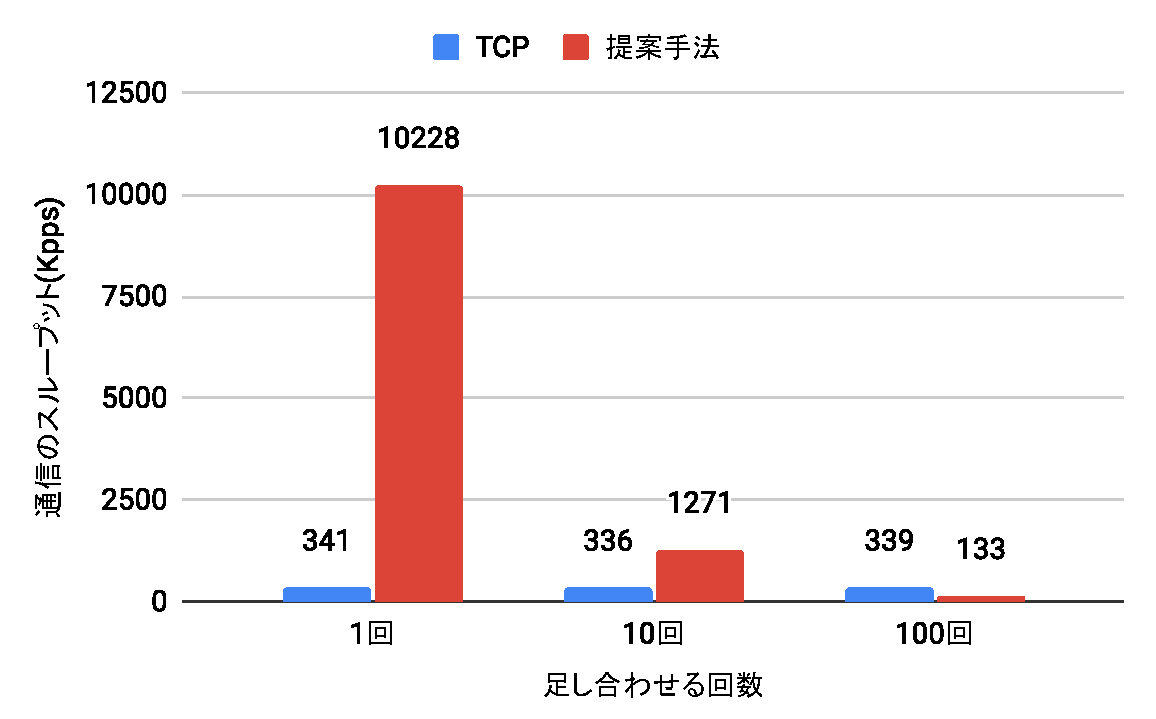
\includegraphics[width=\columnwidth]{pictures/PreExperimentTwoResult.pdf}
  \caption{加算処理の結果}
  \label{fig:PreEvaluationTwoResult}
\end{figure}
